\documentclass[11pt,a4paper]{article}
\usepackage[margin=25mm,headheight=15pt]{geometry}
\usepackage[T1]{fontenc}
\usepackage[utf8]{inputenc}
\usepackage{lmodern,amsmath,amssymb,amsthm,mathtools,bm}
\usepackage{xcolor,graphicx,booktabs,tabularx,array,longtable}
\usepackage{microtype,enumitem,fancyhdr}
\usepackage{xurl}
\usepackage{hyperref}
\definecolor{accent}{HTML}{163B55}
\hypersetup{colorlinks=true,linkcolor=accent,citecolor=accent,urlcolor=accent,
 pdftitle={Affine Lipschitz projections on nearly Euclidean convex bodies},pdfauthor={Matthew J. Colbrook},
 pdfsubject={AIM 898: mathematical result and proof}}
\urlstyle{same}
\setlength{\parindent}{0pt}
\setlength{\parskip}{0.35em}
\setlength{\emergencystretch}{3em}
\setlist{itemsep=0.25em,topsep=0.3em}
\newtheorem{theorem}{Theorem}[section]
\newtheorem{lemma}[theorem]{Lemma}
\newtheorem{proposition}[theorem]{Proposition}
\newtheorem{corollary}[theorem]{Corollary}
\theoremstyle{remark}
\newtheorem{remark}[theorem]{Remark}
\newtheorem{definition}[theorem]{Definition}
\DeclareMathOperator{\Tr}{Tr}
\DeclareMathOperator{\supp}{supp}
\DeclareMathOperator{\Lip}{Lip}
\DeclareMathOperator{\Rea}{Re}
\newcommand{\R}{\mathbb R}
\newcommand{\C}{\mathbb C}
\newcommand{\E}{\mathbb E}
\newcommand{\N}{\mathbb N}
\newcommand{\ip}[2]{\langle #1,#2\rangle}
\pagestyle{fancy}
\fancyhf{}
\fancyhead[L]{\small\sffamily AIM 898}
\fancyhead[R]{\small\sffamily Matthew J. Colbrook}
\fancyfoot[C]{\thepage}
\renewcommand{\headrulewidth}{0.3pt}
\allowdisplaybreaks[2]
\title{\textbf{Affine Lipschitz projections on nearly Euclidean convex bodies}}
\author{Matthew J. Colbrook\\[3pt]
{\small Department of Applied Mathematics and Theoretical Physics}\\
{\small University of Cambridge, United Kingdom}\\
{\small\href{mailto:mjc249@maths.cam.ac.uk}{\texttt{mjc249@maths.cam.ac.uk}}}}
\date{3 November 2026}
\begin{document}
\maketitle
\begin{abstract}
We construct symmetric convex bodies and scalar Lipschitz functions whose canonical affine-projection norms grow at least as the square root of the dimension. The construction persists at any fixed Banach--Mazur distortion greater than one and gives examples with distortion tending to one while the projection norms diverge.
\end{abstract}
\noindent\textbf{Repository target.}
This manuscript concerns AIM problem 898 at revision
\texttt{5d7e26e8444e}. The precise scope is stated below.
\medskip

\section{Main result and proof}
\label{sec:898}

The answer to \cite[Question~19]{HN2019} and the scalar formulation in
AIM~898 is negative.  We construct explicit convex bodies and explicit
$1$-Lipschitz functions for which the canonical affine projection has
Lipschitz constant growing at least as a positive multiple of the square
root of the dimension.

\begin{theorem}\label{thm:898}
There are origin-symmetric isotropic convex bodies
$\widetilde K_n\subset\mathbb R^{n+1}$ of volume one and real functions
$\widetilde f_n$ on them such that
\[
 \operatorname{Lip}_{\widetilde K_n}(\widetilde f_n)\leq1,
 \qquad
 \liminf_{n\to\infty}
 \frac{\operatorname{Lip}_{\widetilde K_n}
       (P_{\widetilde K_n}\widetilde f_n)}{\sqrt n}
 \geq c_*,
\]
where the explicit positive constant is
\[
 c_*=\frac1{26\sqrt{2\pi}}
       \int_{-1}^1(1-z^2)^2e^{-z^2/2}\,dz
       \approx0.0152883.
\]
Consequently no universal finite projection bound exists.
\end{theorem}

\begin{proof}
We begin before isotropic normalization, defining the affine projection
using normalized uniform measure.  For $y\in B_2^n$ set
\[
 h(y)=1-\|y\|_2^2,\qquad c(y)=\frac13\sum_{i=1}^n y_i^3,
 \qquad
 K_n=\{(x,y):y\in B_2^n,\ |x-c(y)|\leq h(y)\}.
\]
Both $h+c$ and $h-c$ are concave on $B_2^n$: their Hessians are
diagonal with entries $-2+2y_i$ and $-2-2y_i$, respectively.
The upper fiber boundary is therefore concave and the lower boundary
convex.  Thus $K_n$ is convex; it is compact with nonempty interior,
and it is origin-symmetric because $h$ is even and $c$ is odd.
Its projection onto the $y$-coordinates is $B_2^n$.  In addition,
$e_0=(1,0,\ldots,0)$ has $K_n$-norm one.

Define the odd $C^1$ function
\[
 \varphi(t)=
 \begin{cases}
 t^3/3,&|t|\leq1,\\
 t-\tfrac23\operatorname{sgn}(t),&|t|\geq1.
 \end{cases}
 \qquad\text{Thus }\quad\varphi'(t)=\min\{t^2,1\}.
\]
Set
\[
 f_n(y)=\frac1n\sum_{i=1}^n\varphi(\sqrt n\,y_i),
 \qquad g_n(x,y)=f_n(y).
\]
Every partial derivative of $f_n$ has absolute value at most
$n^{-1/2}$, so $\|\nabla f_n\|_2\leq1$ everywhere.
Since the $y$-projection of $K_n$ is $B_2^n$, we have
$\|y\|_2\leq\|(x,y)\|_{K_n}$ for every vector $(x,y)$.
It follows that $\operatorname{Lip}_{K_n}(g_n)\leq1$.

We calculate the vertical coefficient of its affine projection.
Let $(\mathsf X,Y)$ be uniform on $K_n$ and put $N=n+4$.
The marginal density of $Y$ is proportional to $h(y)$ on $B_2^n$,
and conditionally on $Y$, the variable $\mathsf X$ is uniform on
$[c(Y)-h(Y),c(Y)+h(Y)]$.  Thus
\begin{equation}\label{eq:898-conditional}
 \mathbb E(\mathsf X\mid Y)=c(Y),\qquad
 \operatorname{Var}(\mathsf X\mid Y)=h(Y)^2/3.
\end{equation}
The distribution of $Y$ also equals that of the first $n$ coordinates
of a uniform point on $S^{N-1}$, because its marginal density is
$(1-\|y\|_2^2)^{(N-n-2)/2}=h(y)$ up to normalization.
The elementary spherical moment formula is
\begin{equation}\label{eq:898-moments}
 \mathbb E\prod_iY_i^{2k_i}
 =\frac{\prod_i(2k_i-1)!!}
 {N(N+2)\cdots(N+2k-2)},\qquad k=\sum_i k_i.
\end{equation}
Odd-coordinate moments vanish, and $(-1)!!=1$.
This formula follows directly by polar integration of the corresponding
Gaussian monomial.

In particular,
$\mathbb E(Y_iY_j)=\delta_{ij}/N$ and
$\mathbb E(\mathsf X Y_i)=1/[N(N+2)]$.
Put
\[
 \ell(y)=\frac1{N+2}\sum_i y_i,\qquad
 r(y)=c(y)-\ell(y),\qquad W=\mathsf X-\ell(Y).
\]
Then $\mathbb E(WY_i)=0$.  Sign symmetry eliminates cross terms in
$\mathbb Er(Y)^2$; using the second, fourth and sixth moments gives
\begin{align}
 V_n:=\mathbb Er(Y)^2
 &=n\left(
 \frac{15}{9N(N+2)(N+4)}
 -\frac{2}{N(N+2)^2}
 +\frac1{N(N+2)^2}\right)\notag\\
 &=\frac{2n(N-1)}{3N(N+2)^2(N+4)}.
 \label{eq:898-residual}
\end{align}
Also $\mathbb Eh(Y)^2=24/[N(N+2)]$.  Consequently
\begin{equation}\label{eq:898-denominator}
 D_n:=\mathbb EW^2=V_n+\frac8{N(N+2)},
 \qquad n^2D_n\longrightarrow\frac{26}{3}.
\end{equation}

Write the canonical affine projection as
$P_{K_n}g_n(x,y)=a_nx+b_n\cdot y$; its constant term vanishes by
central symmetry and oddness.  In coordinates $(W,Y)$ the covariance
of $W$ with all $Y_i$ is zero.  The regression normal equations and
\eqref{eq:898-conditional} therefore yield
\begin{equation}\label{eq:898-coefficient}
 a_n=\frac{\mathbb E[Wf_n(Y)]}{\mathbb EW^2}
     =\frac{\mathbb E[r(Y)f_n(Y)]}{D_n}.
\end{equation}
We evaluate the numerator by a one-dimensional limit.
Let $Z_n=\sqrt n\,Y_1$.  For $i\ne j$, the integrand
$(Y_i^3/3-Y_i/(N+2))\varphi(\sqrt nY_j)$ is odd in $Y_i$,
so its expectation vanishes.  All diagonal terms are equal.  Hence
\begin{equation}\label{eq:898-numerator}
 n^{3/2}\mathbb E[r(Y)f_n(Y)]
 =\mathbb E\left[
 \left(\frac{Z_n^3}{3}-\frac{n}{n+6}Z_n\right)\varphi(Z_n)\right].
\end{equation}

Now $Z_n$ converges in distribution to a standard Gaussian $Z$.
For example, represent the uniform spherical point by independent
standard Gaussians $(G_j)$ divided by their Euclidean norm.  Then
\[
 Z_n\ \stackrel{\mathrm{law}}{=}
 \frac{G_1}{\sqrt{n^{-1}\sum_{j=1}^{n+4}G_j^2}}
 \longrightarrow G_1
\]
almost surely in this coupling by the law of large numbers.
Moreover \eqref{eq:898-moments} gives
\[
 \mathbb EZ_n^8
 =\frac{105n^4}{N(N+2)(N+4)(N+6)}\leq105.
\]
Since $|\varphi(t)|\leq|t|$, this eighth-moment bound gives uniform
integrability of the fourth-degree expressions in
\eqref{eq:898-numerator}.  We obtain
\[
 n^{3/2}\mathbb E[r(Y)f_n(Y)]\longrightarrow
 \gamma:=\mathbb E\left[\left(\frac{Z^3}{3}-Z\right)\varphi(Z)\right].
\]
Gaussian integration by parts twice shows
\begin{align*}
 \gamma
 &=\frac13\mathbb E[(Z^2-1)\varphi'(Z)]\\
 &=\frac13\mathbb E[(Z^2-1)\min\{Z^2,1\}]\\
 &=\frac13\mathbb E[(1-Z^2)^2\mathbf1_{\{|Z|\leq1\}}]>0.
\end{align*}
In the last equality we subtracted the mean-zero variable $Z^2-1$.
The integration by parts is valid for this $C^1$ function with linear
growth and bounded derivative; explicitly,
$\mathbb E[Z\varphi(Z)]=\mathbb E\varphi'(Z)$ and
$\mathbb E[Z^3\varphi(Z)]=
2\mathbb E\varphi'(Z)+\mathbb E[Z^2\varphi'(Z)]$.

Equations~\eqref{eq:898-denominator}--\eqref{eq:898-numerator} now give
\[
 \frac{a_n}{\sqrt n}\longrightarrow
 \frac{3\gamma}{26}
 =\frac1{26}\mathbb E[(1-Z^2)^2\mathbf1_{\{|Z|\leq1\}}]
 =c_*.
\]
Evaluating the projected affine function between $0$ and $e_0$ yields
$\operatorname{Lip}_{K_n}(P_{K_n}g_n)\geq|a_n|$.

Finally choose an invertible linear map $L_n$ taking $K_n$ to an
isotropic body $\widetilde K_n$ of volume one.  Apply the inverse square
root of its positive definite covariance matrix, followed by a scalar
dilation, to obtain such a map.  Set
$\widetilde f_n=g_n\circ L_n^{-1}$.
Normalized uniform measures push forward under $L_n$, and affine maps
are carried to affine maps, so
\[
 P_{\widetilde K_n}\widetilde f_n
   =(P_{K_n}g_n)\circ L_n^{-1}.
\]
Also $\|L_nz\|_{\widetilde K_n}=\|z\|_{K_n}$, preserving both
Lipschitz constants.  On the normalized isotropic body this projection
is exactly the formula in AIM~898.  This proves the theorem.
\end{proof}

\begin{figure}[htbp]
\centering
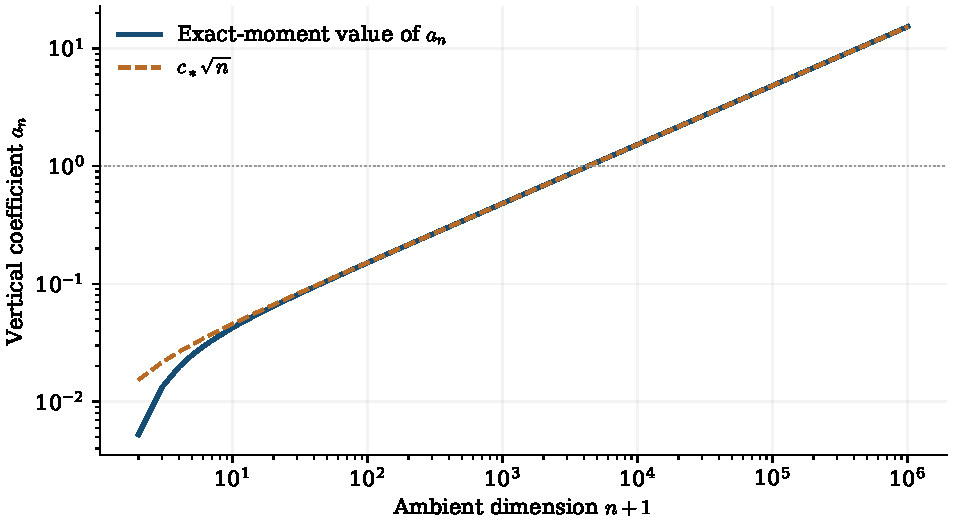
\includegraphics[width=.94\textwidth]{figures/projection_growth.pdf}
\caption{The vertical coefficient $a_n$, a lower bound for
$\operatorname{Lip}_{K_n}(P_{K_n}g_n)$, evaluated from the exact beta-moment
formula. The dashed curve is the proved asymptote $c_*\sqrt n$.
The plotted evaluations illustrate the proof; no numerical estimate
is needed for the unboundedness conclusion.}
\label{fig:898-growth}
\end{figure}

\begin{corollary}[Arbitrarily small Banach--Mazur distortion]
\label{cor:898-near-euclidean}
For every $D>1$, the failure in Theorem~\ref{thm:898} occurs on a family
of normed spaces whose Banach--Mazur distances to Euclidean spaces are
at most $D$.
\end{corollary}
\begin{proof}
Fix $0<\delta<1/2$, and choose fixed parameters
\[
 M\geq\max\{1,(2\delta-\delta^2)^{-1/2}\},\qquad
 0<\alpha\leq\min\{1/2,3\delta\}.
\]
Replace the preceding fiber functions by
\[
 h_M(y)=\min\{\sqrt{1-\|y\|_2^2},\,M(1-\|y\|_2^2)\},
 \qquad c_\alpha(y)=\frac\alpha3\sum_i y_i^3,
\]
and let $K_n^{M,\alpha}$ have fibers
$|x-c_\alpha(y)|\leq h_M(y)$ over $B_2^n$.
Both branches of $h_M\pm c_\alpha$ are concave: the Hessian of
$\sqrt{1-\|y\|_2^2}$ is at most $-I$, the other branch has Hessian
$-2MI$, and $\|\nabla^2c_\alpha(y)\|\leq2\alpha\leq1$.
The minimum of two concave functions is concave.  Thus these are again
origin-symmetric convex bodies.

They satisfy the dimension-independent inclusions
\begin{equation}\label{eq:898-close-balls}
 (1-\delta)B_2^{n+1}\subseteq K_n^{M,\alpha}
 \subseteq(1+\delta)B_2^{n+1}.
\end{equation}
For the outer inclusion, each fiber is contained in a vertical translate
of the corresponding unit-ball fiber, with displacement
$|c_\alpha(y)|\leq\alpha/3\leq\delta$.
For the inner inclusion, write $r=\|y\|_2\leq1-\delta$.
Our choice of $M$ gives
$h_M(y)=\sqrt{1-r^2}$.  Furthermore
\[
 \sqrt{1-r^2}-\sqrt{(1-\delta)^2-r^2}
 =\frac{2\delta-\delta^2}
 {\sqrt{1-r^2}+\sqrt{(1-\delta)^2-r^2}}
 \geq\delta.
\]
This gap absorbs the same displacement $|c_\alpha(y)|$.

Use the identical explicit functions $g_n(x,y)=f_n(y)$ from the theorem;
they remain intrinsically $1$-Lipschitz.  We give the measure comparison
needed to retain the regression asymptotic.  Introduce the reference
body $\overline K_n^{M,\alpha}$ with the same centers $c_\alpha$ and
untruncated half-width $M(1-\|y\|_2^2)$, and let $\overline\mu_n$ be
its normalized uniform measure.  Its marginal $\|Y\|_2^2$ has the
beta distribution with parameters $n/2$ and $2$, exactly as in the
main proof.  The actual body is contained in this reference body and
coincides with it whenever $\|y\|_2^2>1-M^{-2}$.
Writing $a=n/2$ and $\rho^2=1-M^{-2}<1$, the probability of the
exceptional region is bounded by
\begin{equation}\label{eq:898-exponential-tail}
 p_n:=\overline\mu_n\{\|Y\|_2^2\leq\rho^2\}
 =a(a+1)\int_0^{\rho^2}s^{a-1}(1-s)\,ds
 \leq(a+1)\rho^{2a}.
\end{equation}
This decays exponentially in $n$.  Normalized uniform measure $\mu_n$
on the actual body is $\overline\mu_n$ conditioned on that body.
For every bounded function $F$, consequently,
\[
 \left|\int F\,d\mu_n-\int F\,d\overline\mu_n\right|
 \leq\frac{2p_n}{1-p_n}\|F\|_\infty.
\]

Here $|x|\leq M+\alpha/3$, $\|y\|_2\leq1$, and $|f_n(y)|\leq1$,
uniformly in $n$.  All scalar moments appearing in the regression
normal equations therefore differ by $O_{M,\alpha}(p_n)$.
To see explicitly that inversion introduces only polynomial losses,
use coordinate symmetry to write
\[
 u=\mathbb EY_1^2,\quad v=\mathbb E(\mathsf XY_1),\quad
 t=\mathbb E(Y_1f_n(Y)),\quad
 A=\mathbb E(\mathsf Xf_n(Y)),\quad B=\mathbb E\mathsf X^2.
\]
The vertical regression coefficient for either measure is
\[
 a_n=\frac{A-nvt/u}{B-nv^2/u}.
\]
For the reference measure $u=1/(n+4)$; for the actual measure
$u=1/(n+4)+O_{M,\alpha}(p_n)$, hence $u^{-1}=O(n)$.
The two numerators and the two denominators in this formula differ by
$O_{M,\alpha}(n^3p_n)$, which is smaller than every fixed inverse power
of $n$.

For the reference body, the original moment calculation applies with
residual $\alpha r(Y)$ and conditional noise variance
$M^2h(Y)^2/3$.  Its regression numerator is asymptotic to
$\alpha\gamma n^{-3/2}$ and its denominator to
$(2\alpha^2/3+8M^2)n^{-2}$.  The preceding error bounds show that the
actual coefficient satisfies the same limit:
\[
 \frac{a_n}{\sqrt n}\longrightarrow
 \frac{\alpha\gamma}{2\alpha^2/3+8M^2}>0.
\]
The vector $e_0$ still has intrinsic norm one, because
$h_M(0)=1$.  Thus the projection norms are unbounded on the actual
bodies.  Their Banach--Mazur distances to Euclidean space are at most
$(1+\delta)/(1-\delta)$ by \eqref{eq:898-close-balls}.
Choose $\delta$ small enough that this ratio is at most $D$, and apply
the affine normalization from the theorem.  The Banach--Mazur bound and
the projection Lipschitz ratio both survive this normalization.
\end{proof}

\begin{remark}[Distortion tending to one]
The same family can have Banach--Mazur distance tending to one while its
projection norms diverge.  For sufficiently large $n$, take
\[
 \delta_n=n^{-1/8},\qquad \alpha_n=3\delta_n,\qquad
 M_n=(2\delta_n-\delta_n^2)^{-1/2}.
\]
These parameters satisfy the preceding concavity and inclusion conditions.
The inclusions give Banach--Mazur distance at most
$(1+\delta_n)/(1-\delta_n)=1+O(n^{-1/8})$.
Moreover $M_n\sim 2^{-1/2}n^{1/16}$ grows only polynomially, and the
reference probability of the removed region is at most
\[
 (n/2+1)(1-M_n^{-2})^{n/2}
 \leq(n/2+1)\exp(-n\delta_n/2).
\]
All bounds for the moments and the inversion of $u$ in the preceding
proof therefore still introduce only polynomial factors, which are
negligible compared with this exponential decay.  For the reference
measure the numerator is
$\alpha_n n^{-3/2}(\gamma+o(1))$, by exactly the same one-variable
limit as before.  Its denominator satisfies
\[
 \alpha_n^2V_n+\frac{8M_n^2}{(n+4)(n+6)}
 \sim 8M_n^2 n^{-2}\sim4n^{-15/8}.
\]
The actual vertical coefficient consequently obeys
\[
 a_n\sim\frac{3\gamma}{4}\,n^{1/4}\longrightarrow\infty.
\]
The isotropic normalization preserves both this lower bound for the
projection Lipschitz constant and the Banach--Mazur distance.
\end{remark}


\begin{thebibliography}{99}
\small
\setlength{\itemsep}{3pt}

\bibitem{HN2019}
T.~Hyt\"onen and A.~Naor,
\emph{Heat flow and quantitative differentiation},
J. Eur. Math. Soc. \textbf{21} (2019), 3415--3466.
\href{https://doi.org/10.4171/JEMS/906}{doi:10.4171/JEMS/906}.
Questions 10 and 19, and Theorem 9.
\end{thebibliography}
\end{document}
